\section{Pole Figures}

\subsection*{Layout}

% \begin{frame}[fragile]
%   \frametitle{Experimental Pole Figures in \MTEX}

%   \begin{columns}

%     \begin{column}{8.2cm}

%       Characteristics of a single experimental pole figure in \mtex:
%       \begin{enumerate}
%       \item crystal symmetry
%       \item specimen symmetry
%       \item list of specimen directions
%       \item (list of superposed) crystal direction(s)
%       \item (structure coefficients)
%       \item list of diffraction intensities
%       \item background radiation intensities (optional)
%       \end{enumerate}

%     \end{column}

%     \begin{column}{3cm}
%       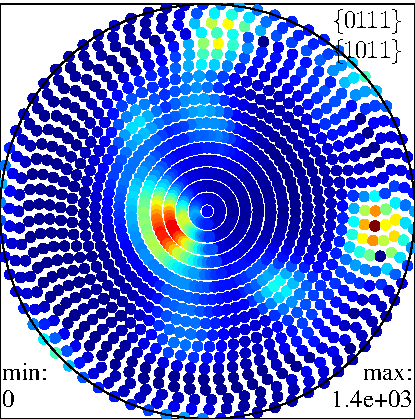
\includegraphics[width=3cm]{pic/pf1}\\
%       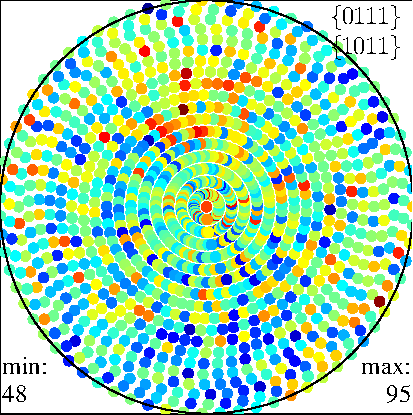
\includegraphics[width=3cm]{pic/pfso9_bg}
%     \end{column}


%   \end{columns}


% \end{frame}


\subsection*{Import Wizard}



\begin{frame}[fragile]
  \frametitle{Experimental Pole Figure Formats supported by \MTEX}

  \begin{columns}

    \begin{column}{5cm}
      \begin{tabular}{ll}
        Fileextension & Format \\
        \toprule
        .ana & EMSE \\
        .axs, .uxd & Bruker  \\
        .cns, .cnv & Dubna\\
        .dat & Geesthacht \\
        .dat, .pwd & D5000\\
        .epf, .gpf &	Popla \\
        .epf, .ppf, .pow &	LaboTEX \\
        .exp, * & Aachen \\
        .ibm & IBM \\
        .jul & Juelich
      \end{tabular}
    \end{column}
    \begin{column}{5cm}
      \begin{tabular}{ll}
        Fileextension & Format \\
        \toprule
        .nja & Seifert\\
        .out & Graz \\
        .plf & Queens Univ. \\
        .ptx, .rpf & Heilbronner \\
        .txt & Philips \\
        .txt & Rigaku Smartlab \\
        .xpe, .xpf & BearTex \\
        .slc & SLC \\
        .xrd, .ras & Bruker XRD \\
        .xrdml & PANalytical XML \\
      \end{tabular}
    \end{column}
  \end{columns}
\end{frame}

\subsection*{Construction (high level)}

\begin{frame}[fragile]
  \frametitle{Importing Pole Figure Data Using a Script}

  \begin{columns}
    \begin{column}{8.5cm}

Script generated by the import wizard:

\begin{lstlisting}
CS = symmetry('-3m',[1.2 1.2 3.5]);
SS = symmetry('triclinic');
\end{lstlisting}

\pause

\begin{lstlisting}
pf_files = {'Q(10-10).cnv',...
            'Q(10-11)(01-11).cnv'}

h = {Miller(1,0,-1,0,CS),...
     [Miller(0,1,-1,1,CS),...
      Miller(1,0,-1,1,CS)]}

c = {1,[0.52,1.23]};
\end{lstlisting}

\pause

      \begin{actionenv}<1-| alert@1->
\begin{lstlisting}
pf = loadPoleFigure(pf_files,h,...
       CS,SS,'superposition',c);
\end{lstlisting}
      \end{actionenv}

    \end{column}

    \begin{column}{3cm}
      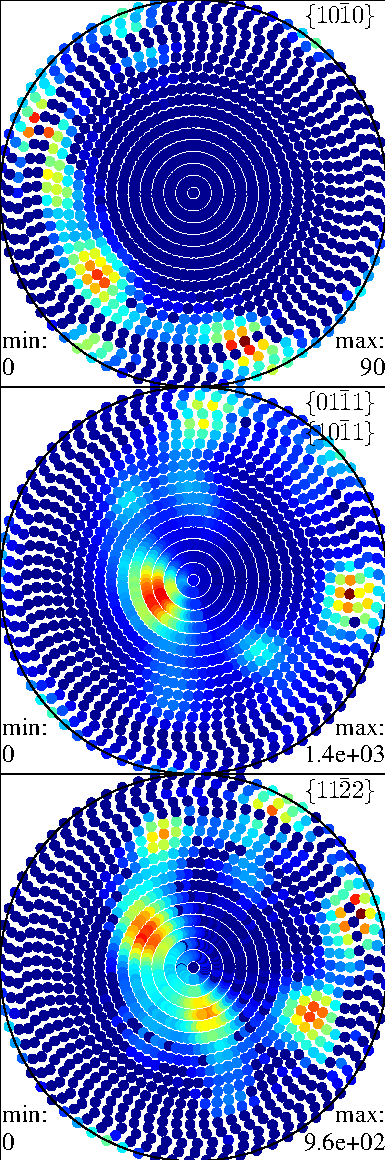
\includegraphics[width=2.5cm]{pic/pforig}
    \end{column}

  \end{columns}

\end{frame}


\subsection*{Analyze Diffraction Data}

\begin{frame}[fragile]
  \frametitle{Using \MTEX to Analyze Diffraction Data}



Retrieve information from pole figures:
\begin{lstlisting}
I = get(pf,'intensities') % intensities
h = get(pf,'Miller')      % Miller indices
theta = get(pf,'polar')   % polar angles
\end{lstlisting}

Basic Statistics:
\begin{lstlisting}
min(pf), max(pf), hist(pf), find_outlier(pf)
\end{lstlisting}

\center{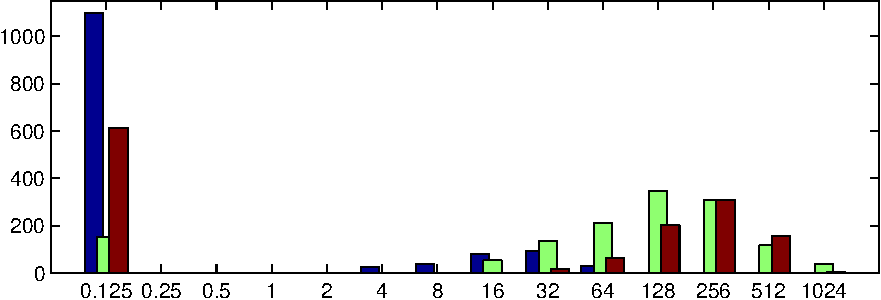
\includegraphics[height=3cm]{pic/hist}}

\end{frame}

\subsection*{Modify Pole Figures}

\begin{frame}[fragile]

  \frametitle{Using \MTEX to Modify Pole Figures}

  \begin{columns}

    \begin{column}{8.5cm}

      Pole figure arithmetics:
\begin{lstlisting}
pf = 2*pf1 + 5*pf2;
pf = [pf1,pf2];
pf = pf([1,3,5]);
\end{lstlisting}

      Pole figure modification:

\begin{lstlisting}
scale(pf,alpha),
union(pf1,pf2),
delete(pf,indices),
rotate(pf,q),
set(pf,'intensities',value,indices)
\end{lstlisting}

      \begin{overprint}

        \onslide<2|handout:1>
        Example:
\begin{lstlisting}
theta = get(pf,'polar');
pf = delete(pf,theta >= 70*degree ...
   & theta <= 75*degree)
\end{lstlisting}
        \onslide<3|handout:0>
        Example:
\begin{lstlisting}
rot = rotation('angle',25*degree,
      'axis',xvector-yvector)
pf = rotate(pf,rot)
\end{lstlisting}
        \onslide<4|handout:0>
        Example:
\begin{lstlisting}
int = get(pf,'intensities');
pf = set(pf,'intensities',1,int < 1)
\end{lstlisting}

      \end{overprint}
    \end{column}

    \begin{column}{3.1cm}
      \onslide<1->
      \only<1|handout:0>{%
        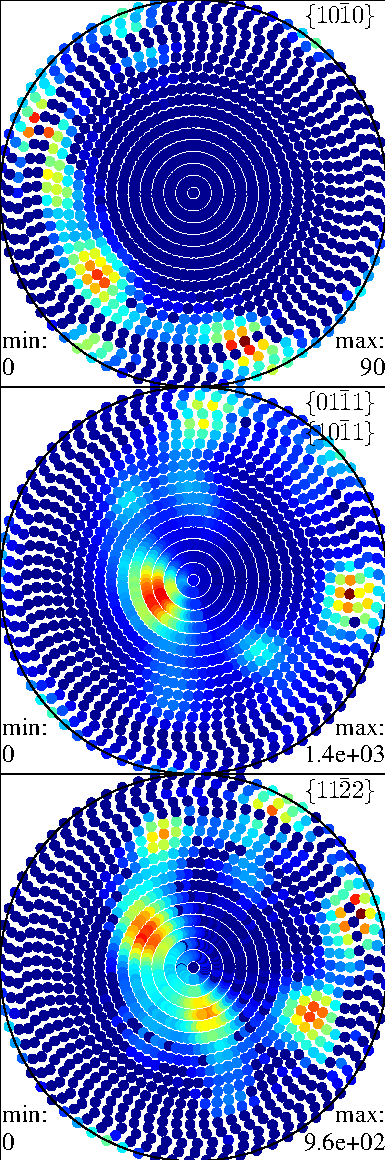
\includegraphics[height=7.5cm]{pic/pforig}%
      }%
      \only<2>{%
        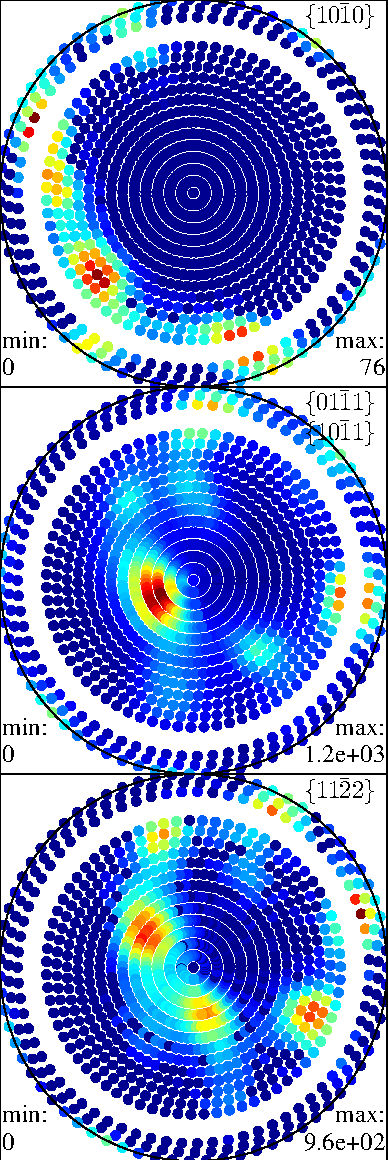
\includegraphics[height=7.5cm]{pic/pfdelted}%
      }%
      \only<3|handout:0>{%
        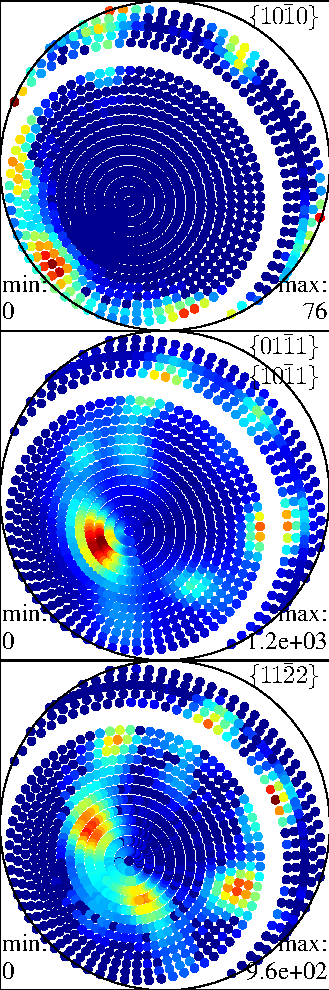
\includegraphics[height=7.5cm]{pic/pfrotated}%
      }%
      \only<4|handout:0>{%
        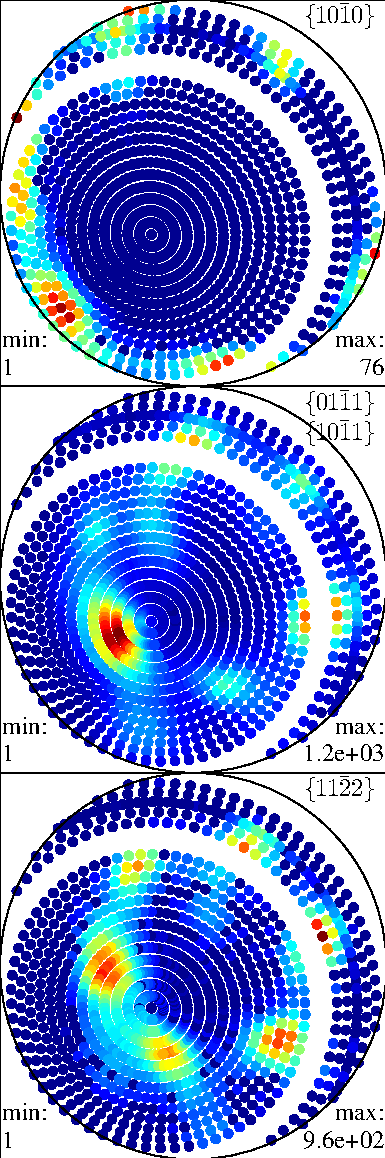
\includegraphics[height=7.5cm]{pic/pfincreased}%
      }
    \end{column}

  \end{columns}

\end{frame}

\subsection*{PDF - to - ODF Reconstruction}


\begin{frame}[fragile]
  \frametitle{PDF to ODF Reconstruction in \MTEX}

  Syntax:
  \begin{alertenv}
\begin{lstlisting}
odf = calcODF(pf,<options>)
\end{lstlisting}
  \end{alertenv}

Options:
\lstset{emph={bandwidth},emphstyle={}}
\begin{lstlisting}
resolution, kernelwidth, bandwidth
iter_min, iter_max
zero_range
ghost_correction
\end{lstlisting}

\pause

\begin{table}[H]
  \centering
  \begin{tabular}{r r r r}
    \toprule
    resolution & kernelwidth  & bandwidth & time \\
    \midrule
    $10^\circ$  & $13.3^\circ$ & 30  & 1s  \\
    $5^\circ$   & $6.7^\circ$  & 58  & 8s \\
    $2.5^\circ$ & $3.3^\circ$  & 121 & 70s\\
    $1.5^\circ$ & $2^\circ$    & 207 & 5min\\
    \bottomrule
  \end{tabular}
\end{table}

\end{frame}


\subsection*{SantaFe}

\begin{frame}[fragile]
  \frametitle{ODF Reconstruction Without Ghost Correction}

\begin{lstlisting}
rec = calcODF(pf_SantaFe,'RESOLUTION',10*degree,...
              'background',1,'iter_max',6)
\end{lstlisting}

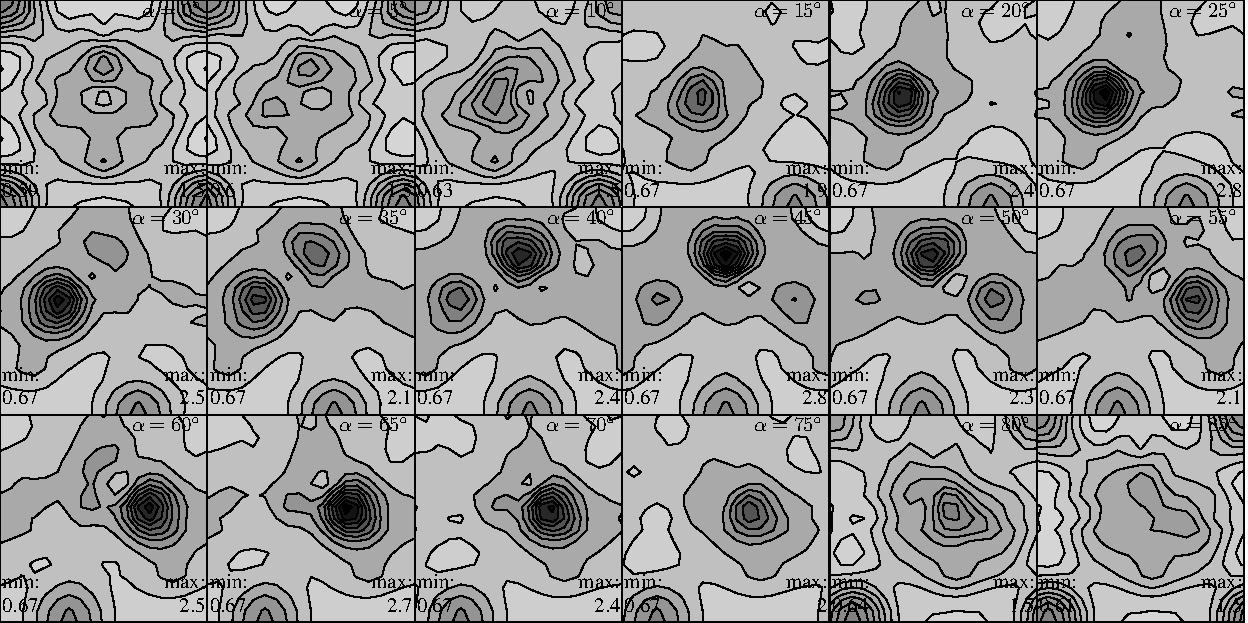
\includegraphics[width=\textwidth]{pic/rec_santafee}

\end{frame}
\subsection*{SantaFe}

\begin{frame}[fragile]
  \frametitle{ODF Reconstruction With Ghost Correction}

\begin{lstlisting}
rec = calcODF(pf_SantaFe,'RESOLUTION',10*degree,...
 'background',10,'iter_max',6,'ghost_correction')
\end{lstlisting}

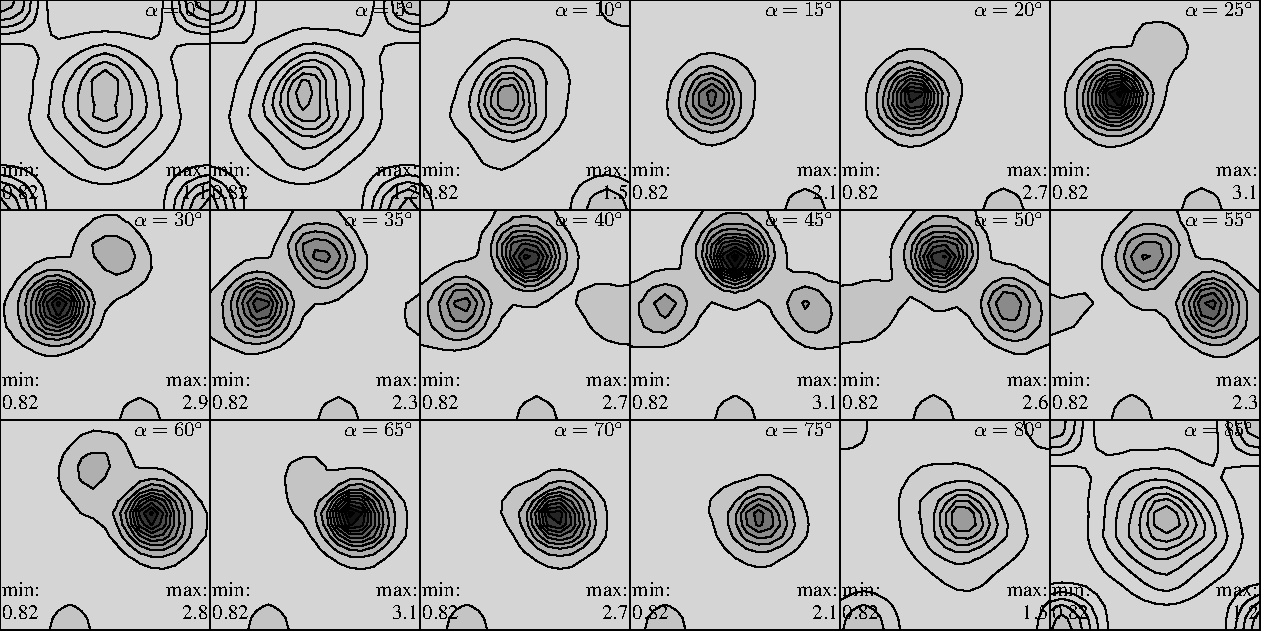
\includegraphics[width=\textwidth]{pic/rec_santafee_ghost_correction}

\end{frame}


\subsection*{Error Analysis}

\begin{frame}[fragile]
  \frametitle{Error Analysis of Reconstructed ODFs in  \MTEX}

Estimate reconstruction error:
\begin{lstlisting}
e = calcerror(pf,odf,<options>)
\end{lstlisting}

Options:
\begin{lstlisting}
RP, L1, L2
\end{lstlisting}

Difference plot:
\begin{lstlisting}
plotDiff(pf,odf,<options>)
\end{lstlisting}

\center{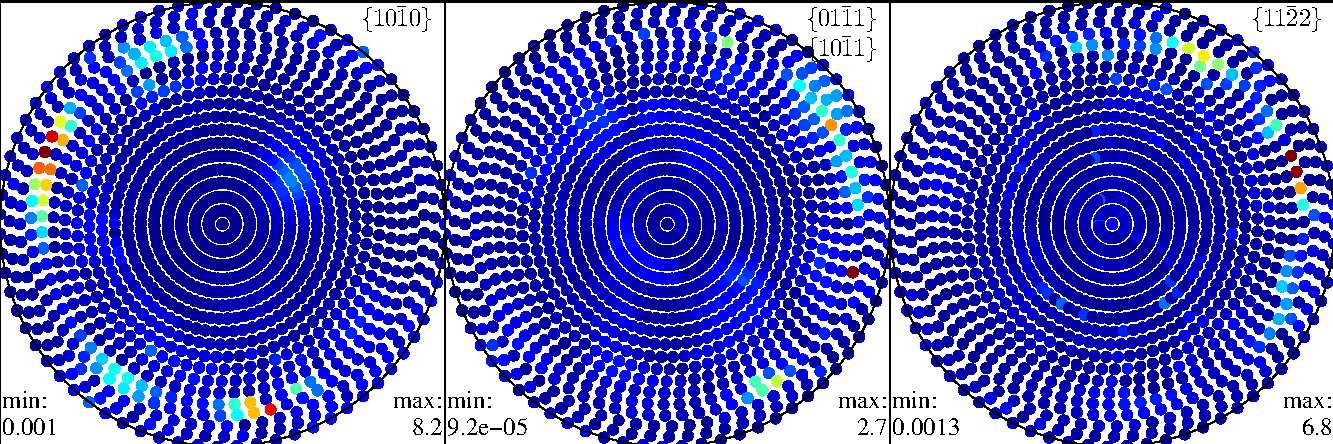
\includegraphics[height=3cm]{pic/diffpf}}

\vspace{3mm}

\end{frame}

% \subsection*{Pole Figure Simulation}

% \begin{frame}[fragile]
%   \frametitle{Pole Figure Simulation in \mtex}

%   \begin{columns}
%     \begin{column}{8cm}

%       Simulation of pole figure data may help to analyze the error made by ODF
%       reconstruction from experimental data.

% \begin{lstlisting}
% %define a model ODF
% odf = SantaFe

% % define crystal directions
% h = [Miller(1,0,0], Miller(1,1,0)]

% % define specimen directions
% r = S2Grid('regular','antipodal')

% % simulate pole figure data
% pf = simulatePoleFigure(odf,h,r)
% \end{lstlisting}
%     \end{column}

%     \begin{column}{4cm}
%       \centerline{
%       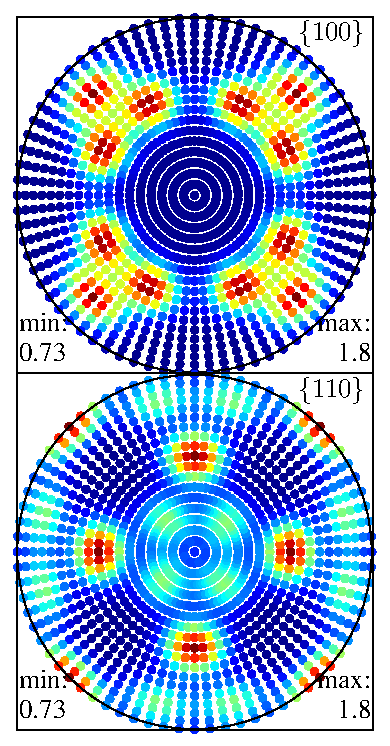
\includegraphics[width=4cm]{pic/simpf}}
%     \end{column}

%   \end{columns}

% \end{frame}

\subsection*{Reconstruction Error}

\begin{frame}
  \frametitle{Reconstruction Error vs. Number of Pole Figures}

  \center{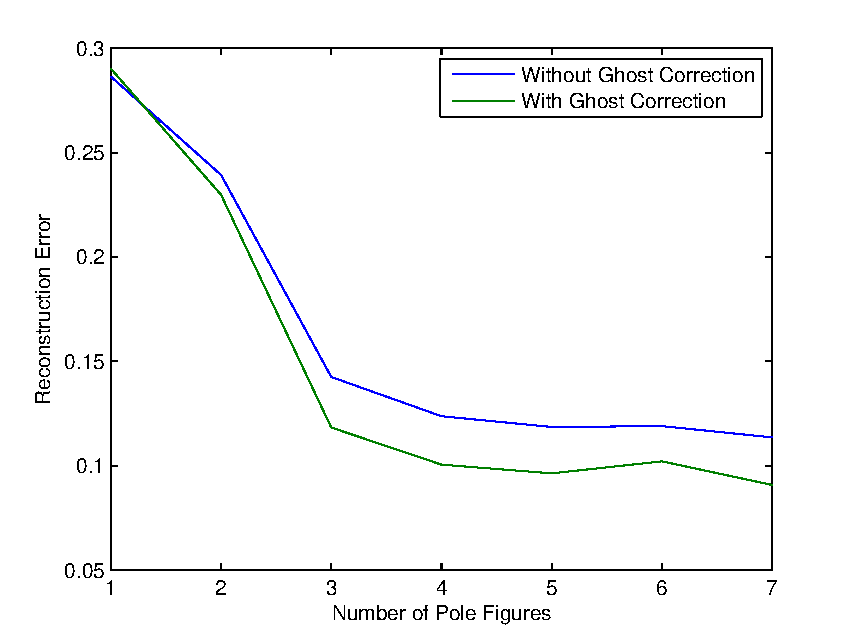
\includegraphics[width=10cm]{pic/pfcorrectness}}

\end{frame}

\subsection*{Exercises}

\begin{frame}

  \begin{Exercise}
    \begin{enumerate}[a)]
    \item Load the pole figure data of a quartz specimen from:
      \texttt{data/dubna}!
    \item Inspect the raw data. Are there problems?
    \item Compute an ODF from the pole figure data.
    \item Plot some pole figures of that ODF and compare them to the measured
      pole figures.
    \item Compute the RP errors for each pole figure.
    \item Plot the difference between the raw data and the calculated pole
      figures. What do you observe?
    \item Remove the erroneous values from the pole figure data and repeat the
      ODF calculation. How do the RP errors change?
    \item Vary the number of pole figures used for the ODF calculation. What
      is the minimum set of pole figures required to obtain a reasonable ODF?
    \end{enumerate}
  \end{Exercise}

\end{frame}


%%% Local Variables:
%%% mode: latex
%%% TeX-master: "main"
%%% End:
